\chapter{Introduction}
\label{chapter:Introduction}


 
\section{Motivation}
\label{sec:intro}
One of the main challenges for nowadays robotics is to bring robots into people's homes and make them help us to perform simple tasks. However, what we consider as a simple task might be very complex for an autonomous system. For example, when setting a table~\cite{iros10kcopman} the robot is likely to be
confronted with a cluttered unstructured scene\footnote{Following the discussion at the Clutter12
workshop at RSS 2012 we acknowledge that this is a ``laboratory clutter'' where the degree of difficulty
is similar to the scenes from the related works but still inferior to the real world clutter.} like the example shown
in \ref{fig:tracking_dists}. In order to interact with an environment like that a robot has to be able to detect and recognize the objects that are on the table. We would like to show that with the ability to interact with an environment robot has a bigger chance to recognize the objects successfully, particularly in the presence of objects of similar colors, shapes and sizes. 


As the initial step for the system we developed an interactive segmentation pipeline that is meant to be used for objects without any texture. In order to show that this is a challenging task that can not be solved with the state-of-the-art perception algorithms we point reader's attention to Fig. \ref{fig:tracking_dists} where we tested three object segmentation algorithms that operate in the RGDB space. Looking at the results we believe that the performance of robot's perception algorithms can be improved, especially in case of: 

\begin{itemize} 
\item textureless objects (all objects in the scene)
\item objects of the same color (a coffee mug and a saucer), 
\item similar shape objects and occlusions (a white and a blue box) 
\end{itemize}

In order to improve the existing algorithms we decided to take use of other properties of the robot. It is easier and arguably more natural to exploit the robot's embodiment
and interaction capabilities in order to obtain a better understanding of its environment.
Reaching out to get a sense of what is around is the way how infants get to know their
``near space'' according to Piaget's theory of spatial cognition in the sensorimotor stage 
(until the age of 2), and getting a hold of connectivity (i.e. object unity) is an important
factor in the infant's understanding of objects at that stage \cite{infants}.


\setlength{\tabcolsep}{0.1em}
\begin{figure}[ht]
%\centering
\begin{tabular}{cccc}
\multicolumn{2}{c}{\multirow{-6}{*}{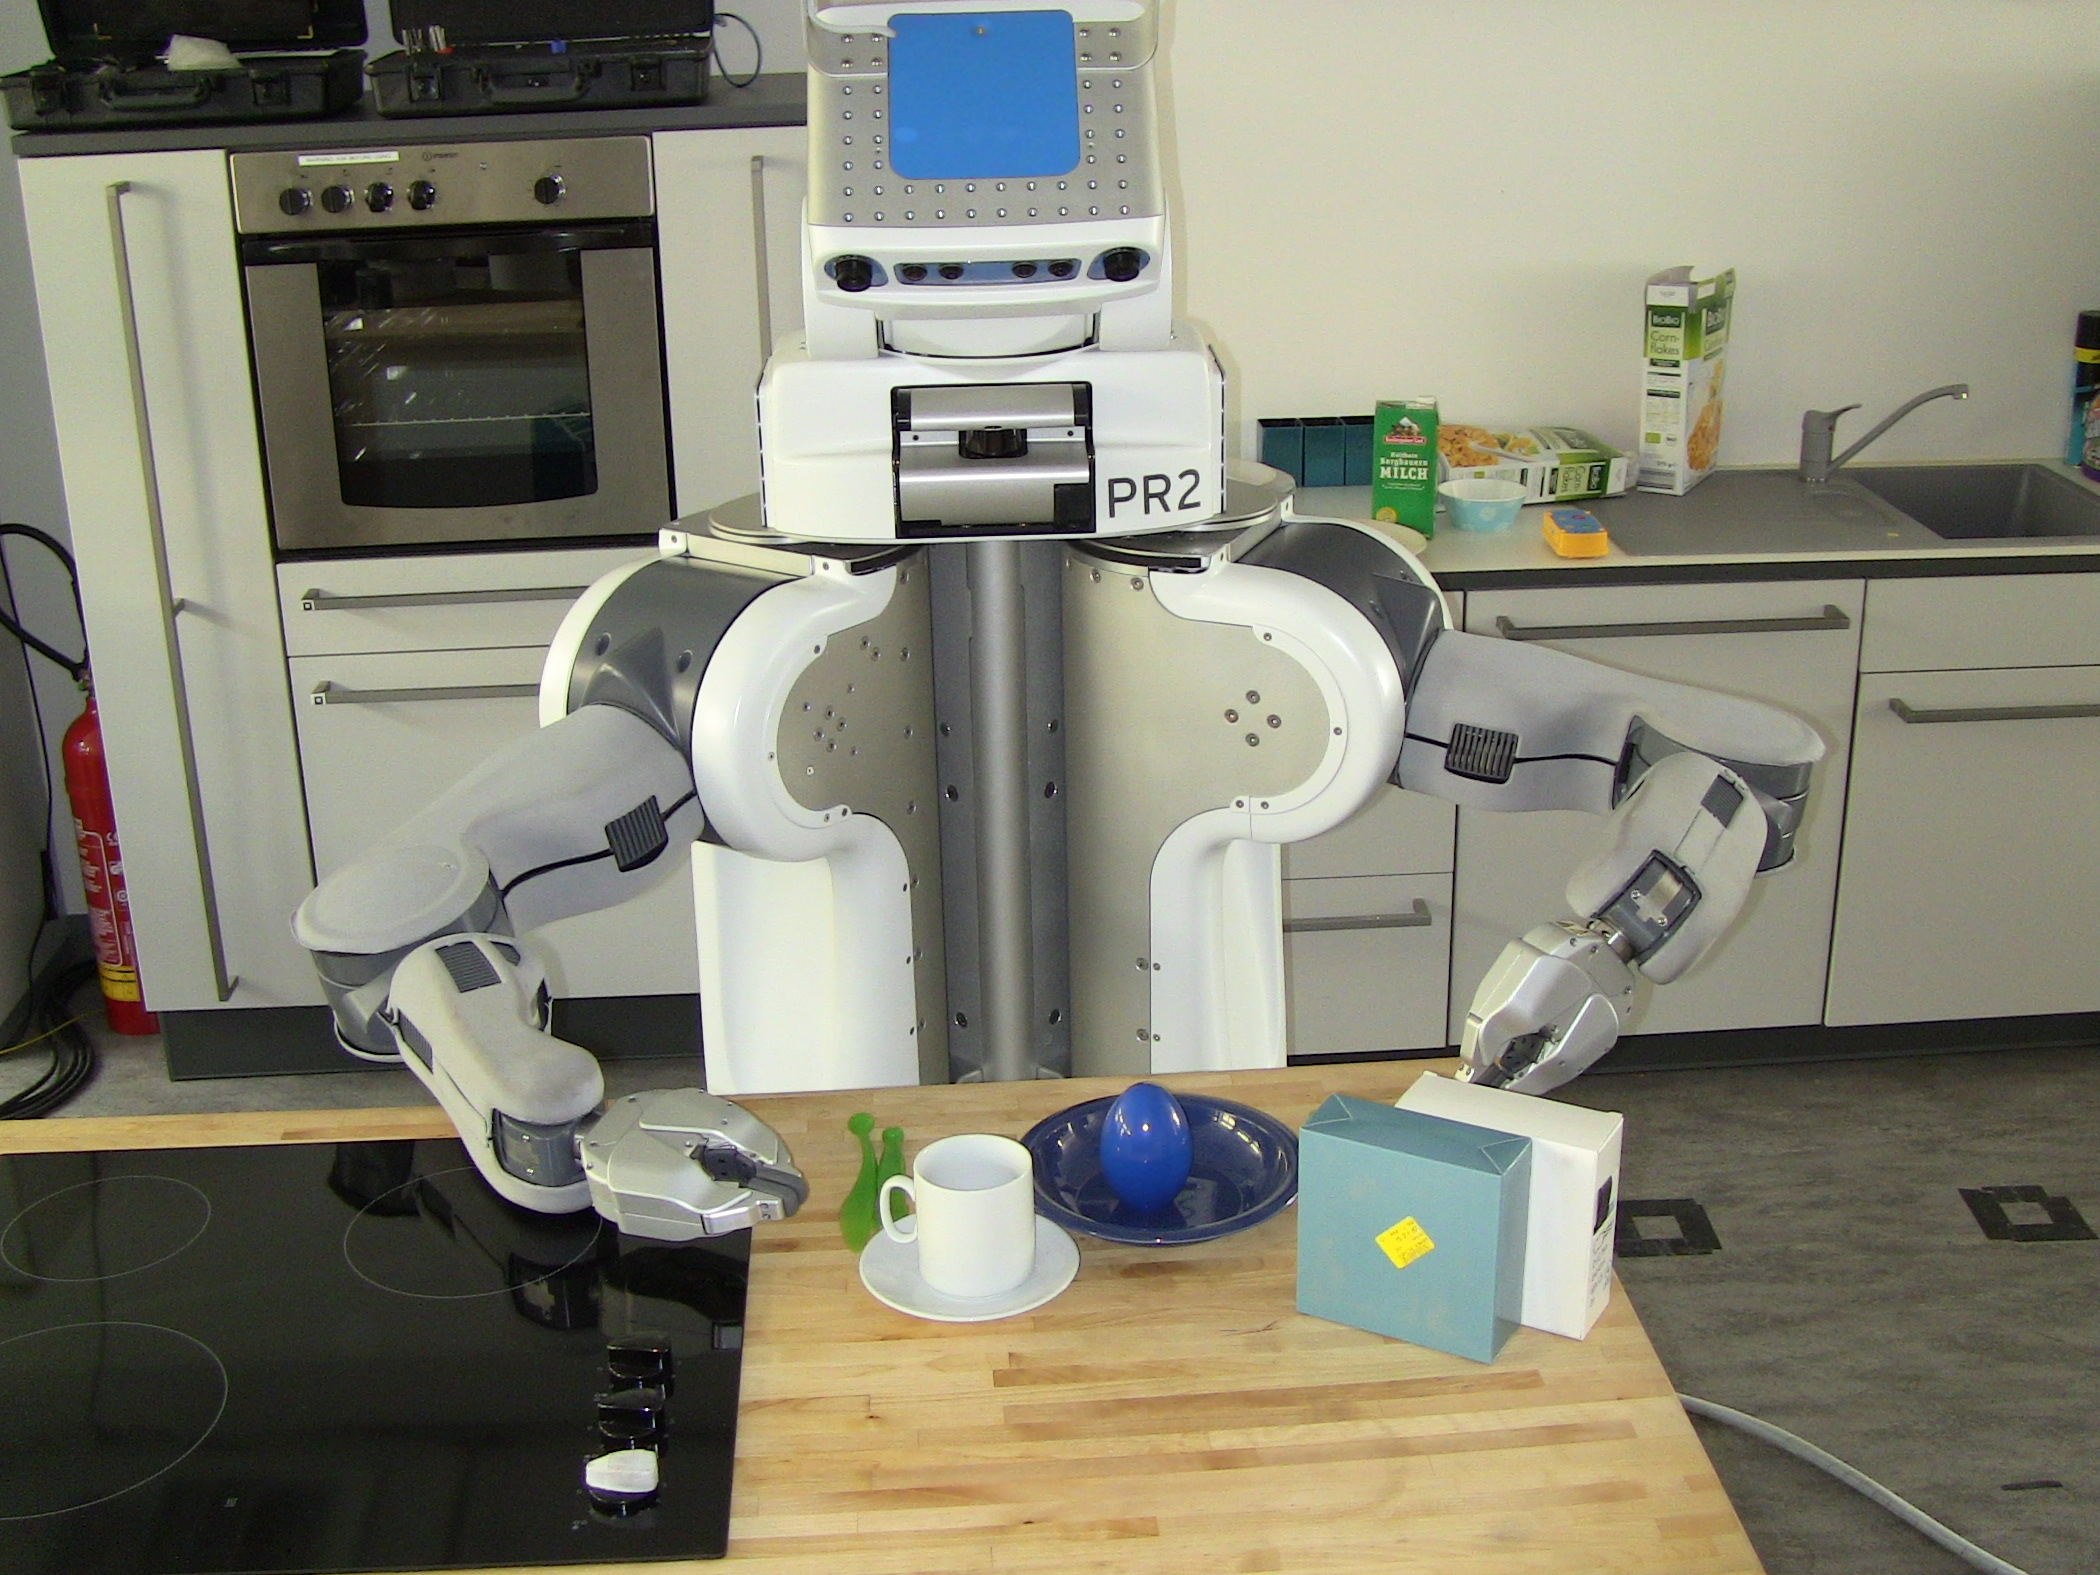
\includegraphics[width=0.5\columnwidth]{figures/teaser/IMG_0395.JPG}
}} & 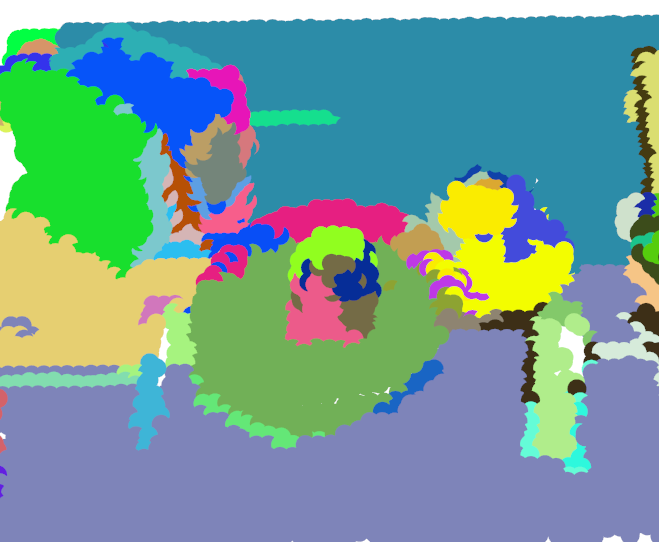
\includegraphics[width=0.23\columnwidth]{figures/segmentation_others/region_growing_rgb.png} 
&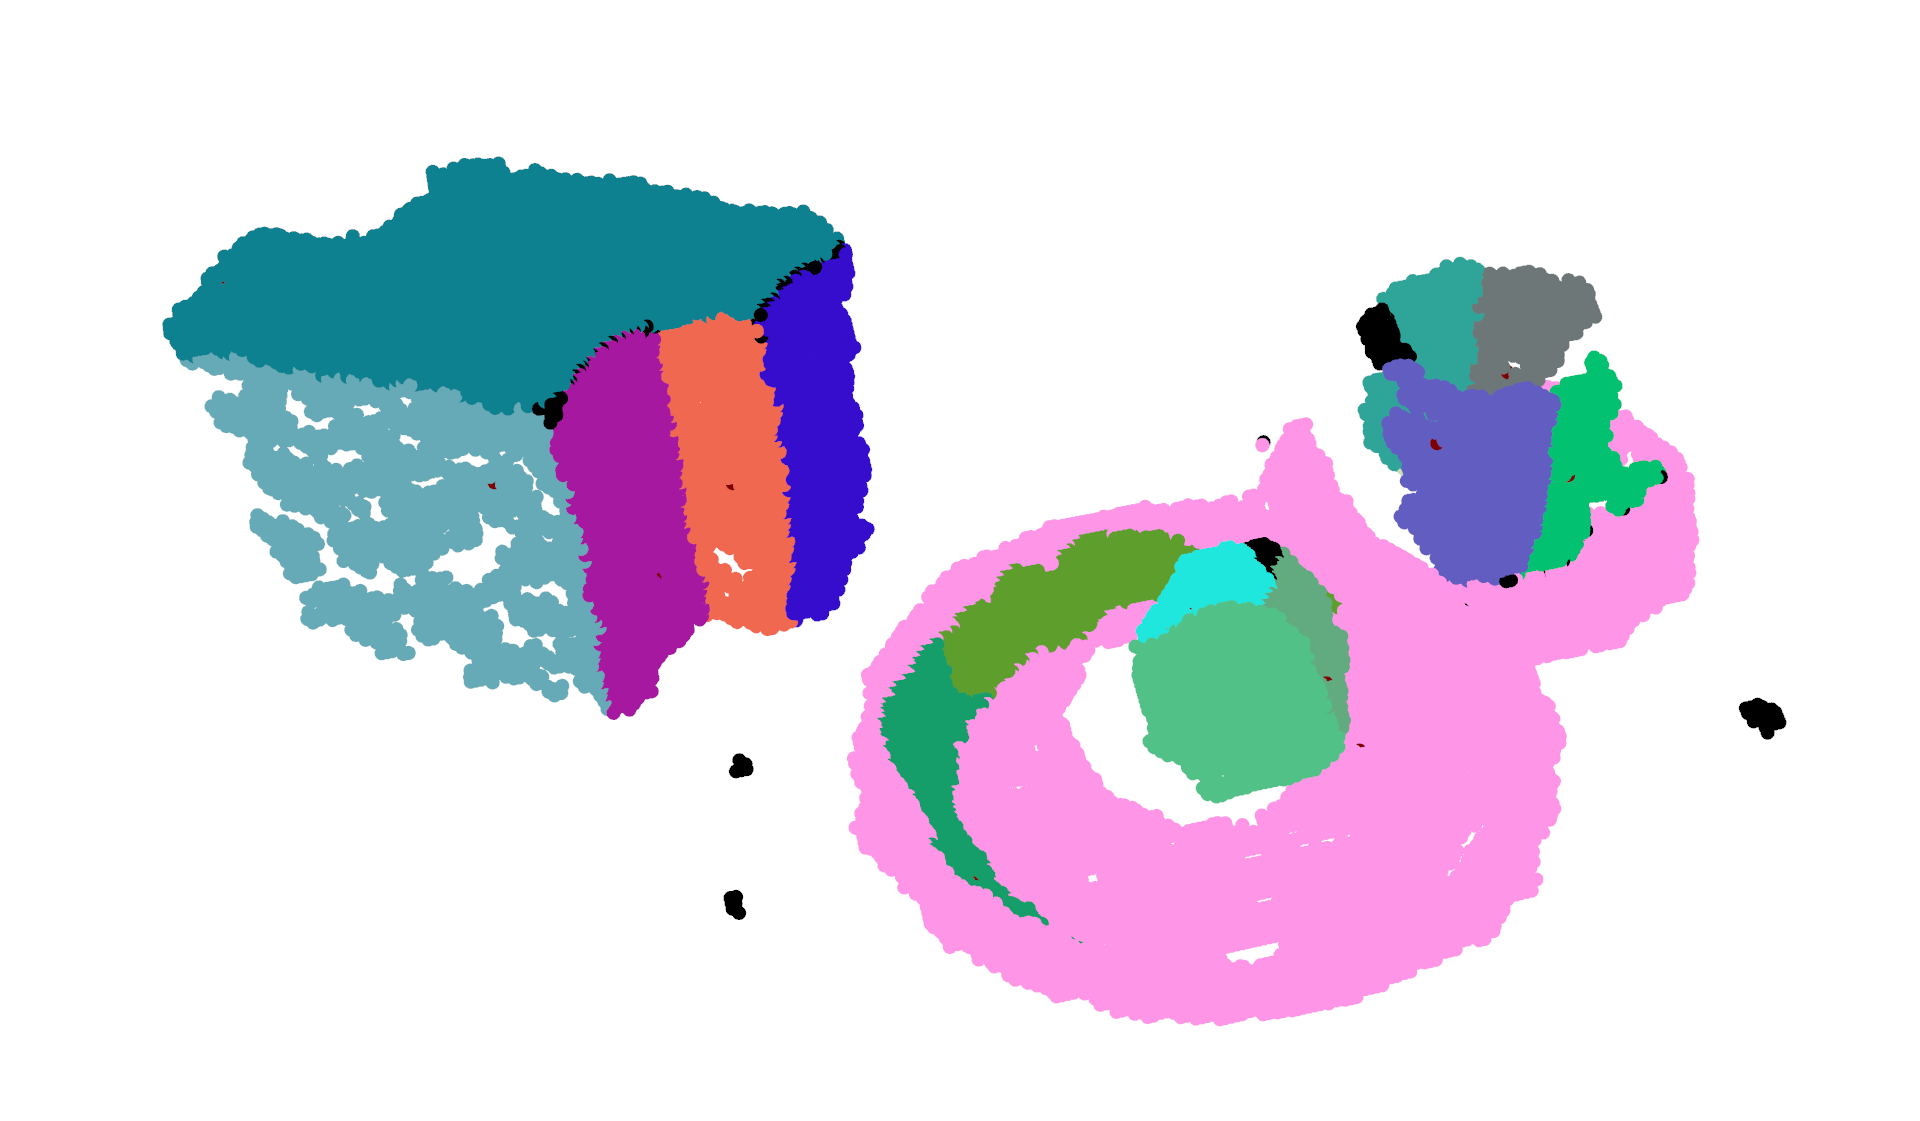
\includegraphics[width=0.23\columnwidth]{figures/segmentation_others/part-graph-hashing.png} \\
\multicolumn{2}{c}{} & \includegraphics[width=0.23\columnwidth]{figures/segmentation_others/graph-based.png} &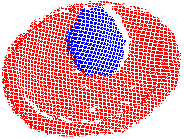
\includegraphics[width=0.23\columnwidth]{pictures/teaser_egg_result-cropped.png} 
%\multicolumn{2}{c}{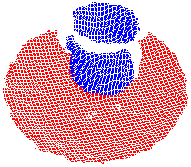
\includegraphics[width=0.38\columnwidth]{pictures/113-cropped.png}} 
\end{tabular}
\caption{Top-left: The service robot PR2 aiming to segment the scene
  consisting of textureless object. Results  of  the   scene segmentation
  using Region  Growing  method~\cite{RGBRegionGrowing} (top-right, NW), Part-Graph-based 
  Hashing~\cite{marton12SC} method (top-right, NE) and Graph-based  
  segmentation method~\cite{Felzenszwalb}   (top-right, SW). These methods work in depth, RGB and RGBD 
  space respectively and all underachieve due to the complexity of this challenging task. 
  On the other hand blue egg on the blue plate was correctly segmented using the interactive approach presented in this paper (top-right, SE)}
\label{fig:tracking_dists}
\end{figure}









\section{Problem definition and goals}

\subsection{Object Segmentation} 

In order to solve the challenge of object segmentation we need to define the terms - image segmentation and object. 

According to L.Shapiro and G. Stockman~\cite{shapiro2001computer}:

"Image segmentation is the process of partitioning a digital image into multiple segments. The goal of segmentation is to simplify and/or change the representation of an image into something that is more meaningful and easier to analyse."

\begin{figure}[ht]
%\centering
\begin{tabular}{cccc}

\multicolumn{2}{c}{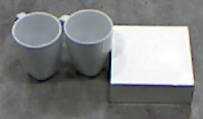
\includegraphics[width=0.45\columnwidth]{figures/3objects/after_push.jpg}}
& \multicolumn{2}{c}{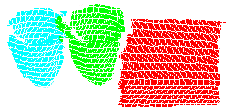
\includegraphics[width=0.45\columnwidth]{figures/3objects/segmented.png}}

\end{tabular}
\caption{Three white objects segmented correctly showing the generality of the apporach for multiple objects.}
\label{fig:three_objects}
\end{figure}


 Following this definition one can conclude that the goal of object segmentation is to segment the image in the way that it is partitioned into multiple objects. However, in our case, as an input we use point cloud data from the Kinect sensor that consists of an image and associated set of 3D points that show 3D structure of the environment. Taking all this information into consideration our goal is to partition a point cloud into multiple objects.

A simple definition of an object in the sense of computer vision problem was presented by A. Mishra~\cite{mishra2012segmenting}:

"A simple object is defined as a compact region enclosed by the depth and
contact boundary in the scene".

According to this definition an output of the object segmentation algorithm would be multiple sets of points that form an object. That is, any point within the set belongs to that object's interior. 

As an example output of the object segmentation we point reader's attention to Fig. \ref{fig:three_objects}. This Figure also shows that even though our experiments were conducted on the set of two objects, the algorithm is generic enough to handle multiple objects. 

\subsection{Object Recognition}
Since the main terms are already defined it is easier to form the problem of object recognition. Once the object is segmented and the robot is aware of its borders it is crucial to be able to recognize what this set of points is. This problem can be understood much wider since we are entering the field of perceptual interpretation. However, in order to keep the problem solvable we understand the recognition of an object as associating the segmented set of points with the data stored in the database of objects. Further implications that stem from information that database contains are not in the scope of this thesis.

\section{Approach} 

In this thesis we concentrate on solving two challenges: 

\begin{itemize} 
\item segmentation of textureless objects since the textured cased was already covered by us in REF. 
\item recognition of objects using interactive perception techniques.
\end{itemize} 

In the next subsections we concentrate on describing our approach with the above mentioned tasks.

\subsection{Interactive Segmentation of Textureless Objects} 


Starting from the former one we would like to show that inducing the motion to the scene can solve the problems depicted in Fig. \ref{fig:tracking_dists}. Similar  to Katz  et al.~\cite{Katz-WS-MM-ICRA2011}, Bergstrom et
al.~\cite{bergstrom11icvs}, and our earlier
work~\cite{bersch12interactive} we propose a system that uses
motion of robot's arm to enable effective
object  segmentation.

Our system consists of five main steps being:

\begin{itemize} 
\item Static object pre-segmentation using part-graph-based hashing ~\cite{marton12SC}
\item Push point estimation using our previous work ~\cite{bersch12interactive}
\item Extraction of RGDB features using point cloud primitives such as lines, corners, cylinders and circles
\item Tracking of above mentioned features using Particle-Filter-based algorithm
\item Graph based trajectory clustering approach
\item Dense model reconstruction based on region growing in normal space
\end{itemize} 


All of these steps are described in details in Chapter \ref{chapter:Textureless Segmentation}. 


There are three important assumptions in our system. First, that each item is a rigid  body and not subject
to large deformations when  interacting with  the robot's  end  effector or
other objects. We also assume that the objects are either flat (box-like) or round (cylinder-like),
which holds for most household objects in publicly available databases~\cite{marton11ijrr}, and
that in the tracking step the features do not get more than $50\%$ obstructed.

The evaluation was performed on 17 scenes with challenging arrangement of flat and
round objects of similar colors, shapes and sizes. $82\%$ of objects
were segmented correctly in these scenes. The interactive segmentation system is available online\footnote{\url{http://www.ros.org/wiki/interactive_segmentation_textureless}} with all instructions needed to install and run it on a real robot. The robot has to have a Kinect sensor as well as at least one arm in order to correctly use the system.

\subsection{Interactive Object Recognition} 

In the second challenge being object recognition we decided to follow the approach presented in the segmentation system. Using our Interactive Segmentation pipeline we have a very good prior for the recognition of objects. Given that the object is segmented correctly we are able to shrink the problem of multiple object recognition to recognition of one currently segmented object at a time. In our system we show that even random rotations and translations can significantly improve recognition of objects.

There are many systems in the field which came up with different solutions to the problem of reliable and robust object recognition. It is commonly believed that the most successful ones were the ones that were based on feature matching approach. All of them encountered to some extend the same problems, among others:

\begin{itemize}
\item features are not fully view point invariant
\item if there is a big difference in lighting between the live image and the image from the database then it is impossible to find correct feature matches
\item features blink a lot because of the not perfect lighting conditions and noise in the image
\item amount of data for one object in the database is very big because the pictures have to be taken from different angles
\end{itemize}

In the chapter \ref{chapter:Object Recognition} we depict the problems and come up with a solution that can partially solve first two of them.
    

















